\chapter{Wstęp i cel pracy (Bogna Lew, Zofia Sosińska)}\label{chap:introduction}

Postrzeganie świata przed erą wielkich odkryć geograficznych znacząco różniło się od tego, które dominuje obecnie. Dawniej
dowódcy nie podejmowali decyzji strategicznych na podstawie precyzyjnych map i pełnej wiedzy o aktualnym stanie zadania,
lecz zmuszeni byli budować przestrzenny obraz istniejącej sytuacji w toku dyskusji z naocznymi świadkami, takimi podróżnicy.
Dobrze obrazującym ówczesne postrzeganie
przestrzeni przykładem jest mapa Imperium Rzymskiego, pokazana na rysunku \ref{fig:mapaIR}. Czytanie jej dosłownie mija się z
celem, gdyż nie są na niej zachowane ani proporcje, ani strony świata. Mimo tego, że basen Morza Śródziemnego został
ówcześnie dosyć dokładnie oddany, “nie wydaje się, aby Rzymianom współczesna kartograficzna wierność była potrzebna” \cite{gbobrektvgry}.
% “Dowódcy opierali się na swojej wiedzy, wiedzy wynajętych przewodników oraz informacjach zwiadowców i tubylców” \cite{gbobrektvgry}.

\begin{figure}[htbp]
    \centering
    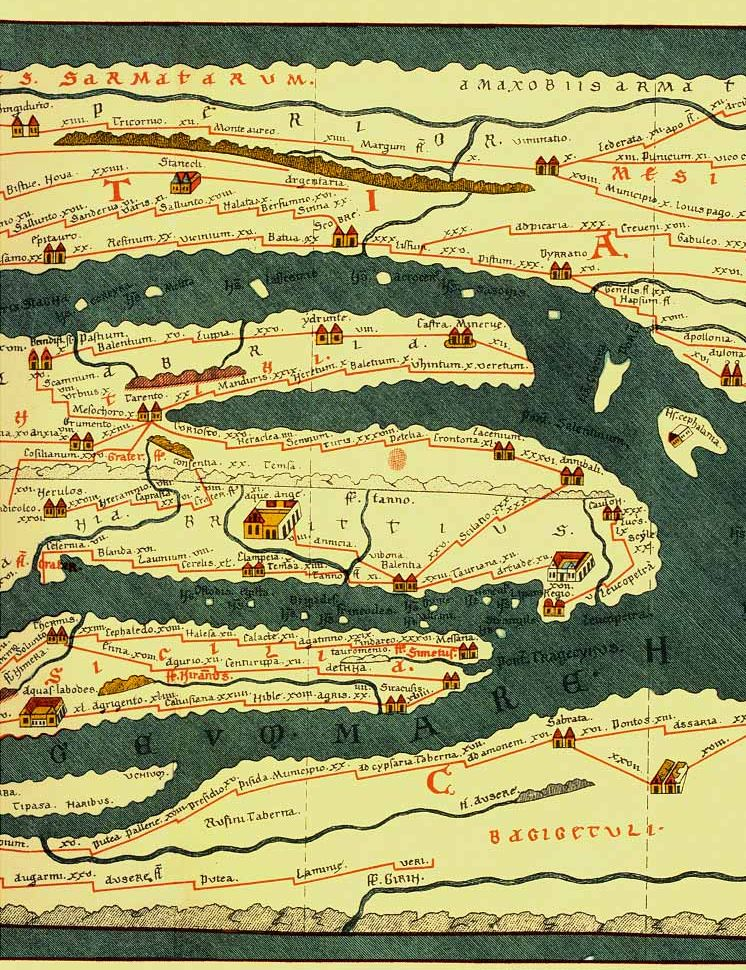
\includegraphics[width=0.5\textwidth]{images/mapaIR.jpg}
    \caption[Mapa basenu Morza Śródziemnego z czasów Imperium Rzymskiego.]{Mapa basenu Morza Śródziemnego z czasów Imperium Rzymskiego\protect\footnotemark.}\label{fig:mapaIR}
\end{figure}
\footnotetext{Internet, \url{https://commons.wikimedia.org/wiki/File:Part_of_Tabula_Peutingeriana.jpg}, dostęp: 05.09.2023}
Aspekt historyczny jest jednym z popularnych motywów w grach komputerowych. Obecnie istnieje wiele tytułów, których
fabuła jest osadzona w realiach historycznych. O takich grach można powiedzieć, że są "formą publicznej dyskusji
pomiędzy projektantem a graczami. Możemy uznać graczy za uczestników chcących wysłuchać argumentów stawianych przez
projekt gry. To też może oznaczać, że postrzeganie czy rozumienie przeszłości przez uczestnika może być kształtowane lub
zmieniane przez ukryty, lub wyraźny argument przedstawiany przez projekt gry" \cite{perception_past}.

Współczesne gry komputerowe, których fabuła osadzona jest w realiach historycznych, stosuje wiele uproszczeń. Ma to na celu poprawienie jakości
rozgrywki gracza, jednakże sprawia, że nie oddaje w pełni realiów. Często obraz dzisiejszych możliwości zasłania faktyczne dowodzenie
w czasach, w których dzieje się gra. Technologia nieznana starożytnym teraz pozwala oficerom na wydawanie rozkazów na podstawie dokładnych map poprzez radio,
jednak w dawniejszych czasach było to niemożliwe. W większości gier historycznych grywalna postać momentami ma wręcz boskie umiejętności i wiedzę. Zwykły człowiek nie był w
stanie w jednej chwili zobaczyć całego świata i wydać komendę jednostkom, znajdującym się na drugim jego końcu, o przemieszczeniu
się do punktu z dokładnością do jednego metra.

Celem projektu jest zaprojektowanie oraz zaimplementowanie prototypowej gry strategii czasu rzeczywistego RTS
(ang. \textit{real-time strategy}) osadzonej we wczesnym średniowieczu z trybem rozgrywki dla jednego gracza. Gra będzie
oferować również elementy typowe dla komputerowych gier fabularnych, co ma stanowić urozmaicenie rozgrywki. 
Udostępniane przez nią mechaniki mają jak najlepiej oddawać realia tamtych czasów, przy
jednoczesnym zachowaniu podstawowych cech tego gatunku. Omówione rozwiązanie powinno zbalansować narzucone ograniczenia tak, aby 
nie pogarszać jakości rozgrywki.

W rozdziale \textit{Wprowadzenie do dziedziny} zostały przedstawione przykłady podstawowych mechanik w grach strategii czasu
rzeczywistego. Kolejny rozdział skupia się na podstawowych narzędziach oraz technologiach wykorzystywanych do wytwarzania
gier komputerowych. Dodatkowo precyzuje wybrane przez zespół środowisko, które zostanie wykorzystane do implementacji
rozwiązań. W następnym rozdziale został przedstawiony projekt wytwarzanej gry. Skupia się on na wizji zespołu oraz
oczekiwanych efektach. Na koniec, w rozdziale \textit{Implementacja} zaprezentowane zostały osiągnięte rezultaty, w jaki
sposób je opracowano oraz efekt końcowy projektu.
